% vim: syntax=tex

%\paragraph{}

%\begin{prose}


%\cleardoublepage
\section*{}
\addcontentsline{toc}{section}{Genèse}
{\em\small
\lettrine[lines=4]{À}{l’origine de ce diwan,} oh oui, il y’avait certes toute l’inspiration qui est y est à l’œuvre, de ces petits riens du quotidiens que l’on ne sait précieux que lorsqu’on les perds. Instants fugaces si bien observés par Bashō qui n’ont d’autre défauts que d’être insaisissables comme l’a relevé Lissān~al-Ḋḋīn, et c’est malgré tout en vain qu’à travers la poésie je comptais en capter un instantané comme l’aurait fait Ȝomār Xayām.

Or, ces infimes détails qui nous rappellent à quel point l’on est vivant et que leur valeur ne s’acquière que par ce fait là, ne peuvent véritablement se jauger qu’à la faveur des deux principales activités de l’homme depuis la nuit des temps que sont l’amour et la guerre. Deux faces d’une même pièce, chacune variante de l’autre. Il est même étrange que nombre de civilisations aient écarté les femmes de la guerre \incise{sauf, hélas, en tant que victimes}, alors qu’authentiquement elles auraient fait d’excellentes stratèges autant que de féroces combattantes.

L’amour est assurément une lutte, tandis que la guerre procède par la séduction. Sun Tzu ne dit-il bien fort à propos \enquote{Faîtes en sorte que vos prisonniers se retrouvent mieux chez vous qu’ils ne le seraient dans leur propre camp} ?

Il y’avait tout cela, dis-je, au fondement de mes quelques vers. Mais en réalités, il n’aurait jamais été pris la peine de saisir le qalām, le stylographe, le porte-plume, ou le clavier, s’il n’y avait pour transcender le tout, ma plus énamourée maitresse, celle qui me tient éveillé toutes les nuits.
}
%\end{prose}

\versehangrightsquare
\poemtitle{Complainte de l’insomniaque}
\begin{verse}
À mes nuits, elle est la plus fidèle amante\\
Puisqu’à nos noces les témoins se sont assoupis.\\
Et si souvent, de ses charmes elle me tente,\\
C’est qu’elle se faufile et se love jusqu’à mon lit.
~
Jalouse, elle évince une à une ses rivales,\\
Verveine, camomille, tisane, aucune ne l’accable.\\
Mais toi, café son acolyte, lui ouvre les volets\\
À chaque fois qu’elle trouve porte fermée.
\end{verse}

\paragraph{}
\begin{prose}
Car enfin, ne vous étonnez pas qu’au toucher, ce livre vous paraisse quelque peu humide, c’est qu’il est tout le long traversé par une intarissable nappe de café.
\end{prose}

\paragraph{}
\begin{prose}
D’ailleurs, c’est devant la porte d’un café où j’attendais quelqu’un que m’apparut le haïku suivant. Au dessus d’un recueil de Bashō que je lisais, se trouvait une bouche d’égout.
\end{prose}

\poemtitle{De la bouche d’égout}
\begin{verse}
La bouche d’égout,
Les jambes de l’élégante
Y ont rendez-vous.
\end{verse}

\poemtitle{De la nappe de café}
\begin{verse}
Sur sillon dorsal,
Fuie la nappe de café
Des cheveux châtain.
\end{verse}

\poemtitle{Du cheveux sur la manche}
\begin{verse}
Café à la main,
Sur la manche de ma veste,
Un cheveux châtain.
\end{verse}

%\paragraph{}
\begin{prose}
C’est plus tard dans la soirée que les vers de Lissān~al\,Ḋḋīn ibn~al\,Xatīb, m’inspirèrent. Ils étaient si à propos qu’ils me semblaient que de son \textsc{xiv}\ieme{} siècle il me les destinait.
\end{prose}

\poemtitle{Flamme dans la nuit}
\begin{verse}
Ô nuit, drape de sombreur nos délits\\
Qui sous le voile noir cueillent un fruit.\\
Ô yeux\endnote{Dans la poésie et la musique arabe, les mots apostrophés \autonym{ô nuit} (\textarabic{يا ليل}) et \autonym{ô yeux} (\textarabic{يا عين}), sont d’ordinaire utilisés comme vocalises.}\label{foot.vocaliseYeuxNuit}, ne soyez  éblouis du feux\\
Qui, ardent, trahi les amants pieux.
\end{verse}

\poemtitle{Parole}
\begin{verse}
Un seul mot sucré d’elle\\
Vaut mieux que mille paroles.\\
Il emprunte aux alvéoles\\
La gelée et le miel.
\end{verse}

\afterpage{\includepdf[pages={1}]{casablanca.pdf}}
\section*{Casablanca}
\addcontentsline{toc}{section}{Casablanca}
\begin{prose}
J’ai dû quitter tôt, trop tôt, cette compagnie pour Casablanca où m’ont appelé certaines affaires. La ville est certes réputée sale et polluée mais par chance j’arrivai un jour où le ciel clair m’inspira le haïku :
\end{prose}

\poemtitle{Du ciel bleu}
\begin{verse}
D’entre les immeubles,\\
Jaillit une vérité,\\
Celle du ciel bleu.
\end{verse}

\begin{prose}
Mais si la beauté providentielle des choses de la nature comme le ciel et les arbres m’émut, je ne manquai pas d’être assailli par les laideurs bien humaines, tan les hommes y rivalisent de vices et de vanités. 

Leur air grave de gens trop occupés semble dire qu’ils s’adonnent à des choses bien grandiloquentes. Voyez-vous, la face un rien grimaçante qui semble vouloir dire qu’ils ont des responsabilités cruciales aux services de renseignement ou qu’ils sont préoccupés par tan de choses du premier ordre ; alors qu’ils ne font qu’essayer quelques petites laines dans une boutique de vêtements ! À en croire leur dégaine cérémonieuse, il s’agirait dans leur façon de se montrer dans des lieux bien vus ou de participer à des mondanités, de rien de moins que d’épopées homériques. Celà  me fit rire.
\end{prose}

\poemtitle{Odyssée consumériste}
\begin{verse}
Ô Ulysse, pourquoi avais-tu quitté ton Ithaque,\\
Si ce n’est pour apporter à ton fils télé et mac ?
\end{verse}

\poemtitle{La ville catin}
\begin{verse}
Casablanca, aussi belle que tes catins\\
Qui, quoique distinctes, racolent en ton sein\\
Dégoûtante comme celles des bas cartiers\\
Princière comme les escortes de Gauthier\endnote{Cartier réputé bourgeois de Casablanca.}
\end{verse}

\begin{prose}
Il y’a bien là force disgrâce et grande hideur mais elle est moins du fait des braves personnes de la classe laborieuse, ceux que quelques esprits malsains et méprisants sont prompts à vilipender.

C’est dans un cartier cossus, aux gens débordants d’une suffisance qui, à la vérité me fit esclaffer davantage qu’elle ne m’indisposa, que m’apparut la mocheté. Celle-ci n’aurait pu être pour moi que motif d’esclaffement et ne pas susciter outre mesure de réflexion, si elle ne manqua d’être grave.
\end{prose}

\poemtitle{La lutte des places}
\begin{verse}
On dit que les bourgeois sont méritants,\\
Que leurs risques valent leurs privilèges,\\
Que de leurs exploits on fait florilège.\\
Rien n’est plus faux, voyons-le sur le champs.
~
Je traverse le passage piéton\\
Quand un bourgeois de soixante-dix ans,\\
Plein d’insolence et de désinvolture,\\
Prétend forcer le passage en voiture.
~
Je l’aperçois me charger le vieillot,\\
Dans son armure de fer, tout penaud.\\
Je le vois, il fonce, je continue.\\
Alors il freine sec sur l’avenue.
~
Bon bah, désolé vieux ça va pas l’faire.\\
Si puissant dans ton armure de fer.\\
Tu t’es arrêté, tout grand manitou,\\
À vingt centimètre de mon genoux.
~
Et bien que fautif, il klaxonne, mécontent.\\
Je vais à sa fenêtre traiter avec lui,\\
Lui, montrer son tort, résoudre le différent.\\
Mais alors ne voilà-t-il donc pas qu’il s’enfuie !
~
Je reconnais là leur légendaire valeur\\
Qui justifie hauts salaires en si peu d’heures.\\
Il y a là du mérite et tan de civisme\\
Qu’il ne s’agit assurément pas d’arrivisme.
~
Ayant agis ainsi avec un prolétaire,\\
Je m’en souviens, un ouvrier de caractère.\\
Il est vrais qu’il était tout aussi effronté\\
Mais voilà, il était resté pour m’affronter.
\end{verse}

\paragraph{}
\begin{prose}
Je passais du reste de nombreuses heures sur les terrasses des cafés où les rayons du soleil m’apportait d’inspirantes pensées.
\end{prose}

\poemtitle[Ivresse à Kaffa]{Ivresse à Kaffa\endnote{Le titre du quatrain est dû au fait que la culture et la boisson du café vit le jour à Kaffa, en Éthiopie.}}
\begin{verse}
Xayam\endnote{L’apostrophe de Xayam, poète bachique iranien, lui rappelle son erreur et instaure une rivalité entre vin et café.}\label{foot.xayam}, il y a grande méprise.\\
Fille de la vigne que tu prise\\
N’est exquise face au chaud ou froid\\
Café qui excite notre émois.
\end{verse}

\poemtitle{L’allier solaire}
\begin{verse}
Je te prierais, à Dieu ne plaise, Aton\endnote{Aton était dans la mythologie égyptienne le dieu disque solaire souvent représenté avec des rayons qui en émanent.}\\
Pour poursuivre ta course dont les rayons,\\
Frappent tout droit et indisposent la belle\\
Contrainte à des postures si criminelles.
~
Pour s’y soustraire un peu et se mettre à l’ombre,\\
Elle recule, se tapis, et se cambre.\\
Mais le long de sa hanche jusqu’à sa croupe,\\
Se trace une courbe d’inédite coupe
\end{verse}

\poemtitle{Du cheveux d’airain}
\begin{verse}
Des cheveux d’airain
Tombant sur les reins.
Et je prend congé du monde
\end{verse}

%\paragraph{}
\begin{prose}
Enfin, avant de m’en aller de Casablanca pour Rabat, une ultime élégante parvint à susciter mon inspiration.
\end{prose}

\poemtitle{La jellaba bleue}
\begin{verse}
Serrée dans sa jellaba de satin,\\
Qui, cintre la courbe pure des reins,\\
D’un ravissant mais étrange contour\\
Quand s’y cale la main sans un détour.

Son tissu, par le hanchement tendu\\
Creuse les belles côtes étendues\\
Et incurve davantage les hanches\\
Enorgueillies et fières de leur danse.

La combinaison qui ses formes cisèle\\
Glisse sur la peau par le ghassoul\endnote{Argile servant traditionnellement à des fins détersives et cosmétiques.} soyeuse\\
Et tombe en cascade d’Akchour heureuse,\\
Ne montrant que les chevilles de gazelle.

Danse jusqu’à éprouver le velours\\
Dont l’agilité sonne les tambours\\
En une flamme bleue qui ternirait\\
L’éclat du cuivre non-halogèné.

Corps des filles de ma patrie et ses contrées,\\
Dans la lave en fusion du Toubkal forgé,\\
De l’Oudaya ou des portes de Tétouan\\
Il est le plus admirable des monuments.
\end{verse}

\section*{Quatre poèmes obscènes et grivois}
\addcontentsline{toc}{section}{Quatre poèmes obscènes et grivois}
\begin{prose}
Décidément, m’étant assis à la terrasse d’un de ces établissements qui font à la fois café et pâtisserie, je ne saurais dire s’il s’agissait de synesthésie, toujours est-il qu’il y’avait dans mes pensées de l’Abi~Nawwās.
\end{prose}

\poemtitle{La pâtisserie}
\begin{verse}

Sucrée est la pétulante qui a l’opéra pour piédestal.\\
Semelle qui de couches de génoise ou de crème de beurre,\\
Et même d’autres nappes d’arômes noisette et de couleurs,\\
A le sommet sculpté d’un toboggan aux courbes cordiales

Sur lesquelles vient s’étaler le pied de meringue\\
Précieusement retenu par les sangles au caramel\\
Et bouté de cinq profiteroles par degré moujingues\\
Aux ongles nappés et vernis de fraises en lamelles.\\

Ainsi juché sur de délicieux talons compensées,\\
Le macaron au bord de la falaise est couronné\\
De la blanche cheville en corne de gazelle,\\
Qui lorsqu’elle se creuse pas à pas, émerveille

Par la démarche des jambes voluptueuses\\
Fuselées de la crème de marron ambrée\\
Capitonnées de mousseline aux mollets\\
Qui fait louvoyer l’amant d’onctuosité.
\end{verse}

\poemtitle{Les boules de glace}
\begin{verse}
Boules pesantes dont le bourrelet déborde,\\
De vanille ou de nougat, sur le cornet\\
Fait de jambes généreuses et fuselées\\
Qui se calent dans la main et s’accordent.

L’abondance fit double ces globes massifs,\\
De crème glacée au rebondissement vif,\\
Dont l’inattendue courbe sait dégouliner\\
Mais sur la saillie un sourire a dessiné.

Poncées par les regards ardents\\
Mandataires des langues alléchées,\\
Les deux se confondant en un sillon\\
Qui creuse d’envie la curiosité.

Le meilleur est encore la pointe du cornet\\
De chocolat ornée ou bien même chaussée,\\
Et craquelle sous la dent comme un pépité\\
\incise{Imagine-t-on}, pour n’en avoir point gouté.
\end{verse}

\poemtitle{L’auguste attribut}
\begin{verse}
Reine de jouissance, à la croupe généreuse,\\
Sculptée et ciselée dans la matière adipeuse,\\
Lorsque son orgueil prend pour trône mon ardeur\\
Souveraine, s’y écrase moelleuse l’épaisseur.
~
Et, étouffant mon exaltation de ses fondement capitonnés,\\
Elle s’y dandine et s’y remue jusqu’à solidement s’y river\\
Pour creuser le canal où se fraye une irrépressible volupté\\
Que l’impérieuse cataracte emplit bientôt avec célérité.
~
Car sans faire attendre l’auguste circonférence\\
Qui, quoique gorgée de richesses débordantes,\\
Donne l’ordre irrévocable de combler son bourrelet\\
De la capricieuse injection qui sait la gonfler.
~
Présidant au devoir d’une pareille majesté\\
Qui par le siège ponctionne le fidèle sujet\\
Soumis à l’autorité des sphères qui caressent\\
Honore sa reine d’aussi agréables tendresses.
\end{verse}

\poemtitle{L’argent du beur et…}
\begin{verse}
La crémière aux gros mamelons,\\
Me donne envie de lui donner du biberon, \\
De l’asperger de tout mon lait, \\
D’être trait comme un goret,\\

Ses yeux de biche,\\
Son regard bovin, \\
Son cul de vache, \\
Ses meuglements 

Derrière son teint de brie frais, \\
Elle sent l’emmental et pue le parmesan \\
Sous son petit tablier hyper moulé, \\
Du maroilles super coulant, 

Quand elle lèche mon \xenism{lben}\endnote{Dérivé du lait dans la cuisine marocaine, obtenu suite au barattage par séparation d’avec le beur.} caillé, \\
L’univers se déchire tout entier, \\
Jusqu’à jaillir sur la voie lactée, \\
Et retomber sur ses joues crémeuses, 

Elle absorbe mes protéines, \\
Je me gave de son calcium,\\
Mélangé et édulcoré à la cyprine, \\
Je l’admire sur un podium. 

Quand elle ouvre sa boutique,\\
On s’y enfonce comme dans du beurre, \\
Elle coagule, se déshydrate, \\
Lorsque je la moule au lait cru.
\end{verse}

\section*{Rabat}
\addcontentsline{toc}{section}{Rabat}
\begin{prose}
Je ne peux hélas rien vous cacher. Dans la \work{Cantate du café} de Sébastien \textsc{Bach}, je suis Lieschen. Que j’aurais voulu être à la maison de café Zimmerman à Leipzig où j’arguerais d’une voix soprano combien  cette boisson est assurément l’ambroisie. Et pour paraphraser Sacha \textsc{Guitry} au sujet, non pas de \textsc{Bach}, mais de \textsc{Mozart}, privilège du délice, lorsque la boisson se tarit, la vacuité était encore d’elle.
\end{prose}

\poemtitle{La boisson}
\begin{verse}
Geste au combien cinématographique\\
Qui du briquet n’envie pas l’esthétique.
 
Saisissant la tasse à la belle croupe,\\
C’est aux cieux que je lève cette coupe
 
Pour l’élégance, je porte à la lèvre avide\\
mon verre de café depuis bien longtemps vide.
\end{verse}

\cofeAm{0.2}{0.5}{-20}{1.5cm}{-2.5cm}
\begin{prose}
J’écrivis les lignes qui suivent alors que j’étais attablé à un établissement de l’avenue Patrice Lumumba, en plein milieu d’une harassante journée de travail, tandis que le soleil caressait de quelques rayons dont la rigueur pouvait s’épargner pour peut que l’on s’en convainquit.
L’une de ces étranges journées où l’ensoleillement se trouve dans un équilibre précaire qui daigne accorder, à condition d’application mental, aux hommes le choix entre les douceurs d’une chaleur avenante et les morsures scélérates d’un brulant incendie.

Je me souviens que ce jour là, comme à mon habitude, je me mis à la table proche du palmier d’où de temps à autre tombaient quelques noies dont le bruit de la chute faisait un agréable tapotement. Je noyais alors ma fatigue dans un café noir qu’accompagnait un onctueux paris-brest (la chose a son importance). Mais, trêve de \xenism{story-telling} qui tourne à l’exhibition d’une \xenism{instagrameuse} pré-pubère \incise{quoiqu’il me faut vous expliquer impatients lecteurs ces conditions}. Toujours est-il que je laissais couler les précieuses gorgées du seul et véritable or noir lorsqu’arriva splendide une jeune femme dans sa démarche majestueuse qui, en osmose avec les tons beige, ambré et alezan de la décoration du lieu, par une soudaine synesthésie risqua de me la faire confondre avec ma boisson.

En un laps mon esprit vacilla et ne pu honnêtement plus distinguer ces deux entités, tant il y’avait là identité. Et les rayons ardent de l’archer héliaque haut juché qui jusqu’à lors trébuchaient sur ma cuirasse dermique parvinrent, à la faveur d’une faiblesse naissante, à me transpercer la peau. M’épongeant le front, il me fallut par de laborieux efforts me ressaisir mais ce fût alors au prix d’une contrepartie des plus voluptueuses. Que tous les incidents, différents, discordes, et difficultés puissent se résoudre de la sorte\,!

Car raisonna en mon esprit une entrainante musique qui voulu clamer, par les joyeuses percutions d’une fanfare, la gloire de l’arrivée de cette belle, et dont les paroles me vinrent naturellement, comme dictées par la nécessité de célébrer une suavité fière qui ne pouvait souffrir aucune patience. Plût au Ciel que mon lettrisme eusse pu suffire à transcrire le solfège afin de vous apporter l’air que j’entendis. Mais si je ne peux vous rapporter le son alors au moins ne vous laisserais-je ni aveugle, ni anesthésique, ni même agueusique  de la peau de cette élégante quoique portant un voile faisant des pétales de caféiers autour de son pistil de visage (je sais le lieux commun éculé depuis Gérard \textsc{de Nerval} mais il est ici irrésistible), qui me sembla aussi onctueuse que la mousseline de mon paris-brest tandis que la fierté que l’on lisait dans ses yeux rivalisait d’âcreté avec le café.

Il y’avait grande adresse dans la lenteur pourtant célère de ses mouvements souples qui nous confinent à l’oxymore. Jambe après jambe, elle faisait accorder sa taille élancée au balancement de  ses épaules dans un rythme si parfait que j’en fus bouleversé. Un évènement eu lieu ce jour là. Je pourrais encore poursuivre sur la description du ravissement qui fût mien et vous dire que le soir même en fait de mon entrainement quotidien aux armes, ce fût un qalām dont l’encre, tel que le rapporte le ĥadith, est plus sacrée que le sang du martyr, que je dû encocher à mon arc lorsque je  me précipitais le soir même pour peaufiner et ciseler encore ce poème qui me teint éveillé jusque tard dans la nuit. C’est que cette dame se confondit avec la boisson qui excite jusque dans ses effets métaboliques.
\end{prose}

\poemtitle{La ravissante boisson}
\begin{verse}
Puissant arôme subtile,\\
Sans lequel tout est futile,\\
Toi qui enchante mes sens\\
Pareil à la belle qui s’avance,
~
Toi qui fait jalouser l’ambroisie,\\
Que le bachique\endnote{Voir note \ref{foot.xayam}.} ne sait suspecter,\\
Exhale les licites parfums d’Andalousie\\
%De Kaffa,
%de Florence,
%de Vénétie,\\
%D’Ankara,
%de France,
%et de Tunisie,\\
Qui haut hissent nos gobelets,
~
\BrText{%
Et coule, coule le long de ma gorge.
Abreuve-moi élégante de tes ombres
Qui naviguent dans ton corps sombre,
Ce métal en fusion dans la forge.
\,
Ondoie, flamme singulière,
Lorsque le vent frais te flaire,
De tes torrents de charme
Qui torréfient mon âme.
}
~
En place du véritable or noir,\\
L’huile de pierre\endnote{L’\autonym{huile de pierre}, décrite au vers précédent comme \autonym{or noir} est le pétrole.}\label{foot.huiledepierre}, en imposture,\\
Se dressa pour se faire voir,\\
Mais ne peut en emprunter l’allure.
~
Car si du nectar du désert\endnote{Voir note \ref{foot.huiledepierre}.}\\
La vile engeance prolifère,\endnote{Allusion à l’aphorisme selon lequel \enquote{les conflits prolifèrent dans les zones pétrolifères}.}\\
\cofeDm{0.1}{0.1}{0}{0cm}{0cm}
De tes arômes apaisantes\\
Nous ne vîmes que l’entente.
~
\emph{Refrain}
~
Et suit de tes odeurs enivrantes\\
La procession imminente de la reine\\
À la couronne sertie de tes graines\\
Qui du caroubier\endnote{Les graines de caroubier, du fait de leur masse extrémement régulière de 22\,g, servirent d’étalon dans la joyairie et fondèrent l’unité du carat.} a ravi la patente.
~
Que le barista actionne son levier\\
\cofeDm{0.1}{0.5}{5}{-7cm}{0cm}
Et le serveur diffuse ton encens.\\
La voici, au chemisier de lait,\\
Dans sa démarche quintéscenciée.
~
\emph{Refrain}
~
Traversant les rangées de table sur la cours,\\
Sur mes lèvres, coule lisse ta robe de velour.\\
Et dans mon verre se projette en noir la vidéo\\
Tandis que tes flots se font ouïr en dolby stéréo.
~
Amante, tu es la sultane vivante\\
Qui domine cette maison de café\\
Des sveltes volutes odorantes\\
Qu’imprime ta démarche rafinée.
~
\emph{Refrain}
~
Orbe fluide, à toi la grâce et à moi l’ivresse.\\
Latte macchiato au chemisier blême,\\
Tes mouvements emplis de promesses\\
Incitent nonchalamment ma lente plume à déborder du poème.
~
Et d’Adam et Ève dont nous connûmes l’errance\\
Qui sacrifièrent l’Éden entier au seul pommier,\\
Meilleur compte eurent il eu de ponctionner le Rubiacé\endnote{En l’occurrence le caféier qui est de la famille des Rubiacés.}\\
Car celui-là seul est l’arbre de la connaissance.
~
\emph{Refrain}
~
Tu m’hôte le sommeil, m’éveille, m’extasie,\\
Et m’attire de ton lien dans la nuit\\
Où la noirceur de l’espresso céleste\\
N’est parsemée que de sucre leste.
~
Lorsque du voile tu te déleste,\\
Je crois voir du liégeois la crinière\\
Napée de caramel qui en un geste\\
Trouve de ma bouche l’itinéraire.
~
\emph{Refrain}
\end{verse}

%\paragraph{}
\begin{prose}
Là, je fis une rencontre, assurément des plus charmantes, celle de mademoiselle F***.
\end{prose}

\poemtitle{Bout des doigts}
\begin{verse}
Lorsqu’à peine de ses doigts elle m’effleure.\\
Ô nuit, ô yeux, ô yeux, ô nuit\endnote{Voir note \ref{foot.vocaliseYeuxNuit}.}\\
C’est une pluie qui ravit par sa fraîcheur.
\end{verse}

\poemtitle{Fruits rouges}
\begin{verse}
Myrtille, framboise, fruit de la passion,\\
Dégustons les délices de l’instant de braise.\\
Sans le moindre égard pour tous les qu’en-dira-t-on,\\
Nous croquerons bien encore cerise et fraise.
\end{verse}

%\paragraph{}
\begin{prose}
Je promis à F*** de venir la voir à Eljadida dès après \fallbackserif{Ȝ}īd al\,Aḋĥā.
\end{prose}

\begin{prose}
Mais pour l’instant, sous les murailles de la vieille ville de Salé, m’apparurent de jeunes filles qui quoiqu’emmitouflées dans des haïks, n’en demeuraient pas moins coquette avec leurs vêtements contemporains en dessous. D’improbables chaussures à talons aux couleurs vives pointaient même… un clapsus faillit me faire écrire \enquote{piédestal}.
\end{prose}

\poemtitle{Haïk}
\begin{verse}
Soutenant du dessus du blanc litham\endnote{Bande d’étoffe couvrant la partie basse du visage des femmes, juste en dessous des yeux.}\label{foot.litham}\\
Un regard insolent de peccadille.\\
Mystère du tissus qui déshabille\\
Davantage qu’il ne vêtit les femmes.

Triangle facial de chaire blanche\\
Au haut pyramidion capillaire\\
Est peau de chagrin pleine de lumière\\
Où s’agrippent de lestes espérances.

Cette obscénité qui se fit pudeur\\
Serti le visage décolleté,\\
Et à l’endroit où l’on retient l’ardeur\\
Crée une si nouvelle nudité

Où la pupille qui pointe en téton,\\
Aréolée de khôl. Quand il se baisse,\\
Soustrait aux regards ses délicatesses,\\
Opposant des sourcils en un auvent.

Et sourcils effilés jusqu’au canthus,\\
En un ongle lacérant ma poitrine\\
Qui est alors l’âtre ou siège chagrine\\
La flamme aux feuilles tissées de lotus.

Resplendissants et glorieux visages,\\
Pistils des femmes emplis de présages\\
Aux cheveux sépales qu’elles cajolent,\\
Se sont-ils adjoint pareilles corolles ?
\end{verse}
\afterpage{\includepdf[pages={1}]{haik.pdf}}

\poemtitle{Des cliquetis}
\begin{verse}
Cliquetis claudiquent
Sur le cadran métallique
Avec conséquence.
\end{verse}

\section*{Forêt}
\addcontentsline{toc}{section}{Forêt}
\begin{prose}
Je me rendis à la forêt de Mamora, non loin de Kénitra où je pu m’exercer à l’arc, peut avant \fallbackserif{Ȝ}īd al\,Aḋĥā.
\end{prose}
\poemtitle{Entrée du fauve}
\begin{verse}
Des crocs scintillants\\
De la Bête menaçante,\\
La vallée de larmes.
\end{verse}

\poemtitle{L’archer forestier}
\begin{verse}
Ricoche brutale flèche d’airain,\\
Sur la roche solide du sapin,\\
Comme le boulet de l’artillerie,\\
Qui sur la fière tour  ronde dévie.\endnote{En architecture militaire médiévale, les tours à base ronde sont connues pour être plus résistantes, notamment face au tirs d’artillerie, que les tours à base carrée.}\label{foot.tourRonde}
~
Mais de sève de Salicacées saturée\\
Enfonces-toi dans l’essence du peuplier\\
Qui au retour en laisse la pointe souillée\\
Et âcre d’une jaunâtre viscosité.
~
Si les arbres ne peuvent nous contenter,\\
Tournons-nous alors et pointons le palmier\\
Dont le stipe amoureux accueille d’égards\\
Quoique, jaloux, retient fermement le dard.
~
Reste donc le chêne-liège doux de bois\\
Qui, quoique par cette saison démasclé,\\
Est la  cible dont le tissage parfait\\
Prend la flèche et me laisse la retirer.
\end{verse}

\poemtitle{Du komorebi}
\begin{verse}
Branches de forêt,
Le soleil sait s’y frayer
D’inattendus gués.\endnote{Le \xenism{komorebi} est dans la culture japonaise, le phénomène visuel par lequel les rayons du soleil se faufilent à travers les branches des arbres.}
\end{verse}

\poemtitle{De l’abeille}
\begin{verse}
L’abeille grappille.
Posée sur la camomille
Est grain de beauté.
\end{verse}

\poemtitle{Caresses de l’oud}
\begin{verse}
À la première caresse de l’oud,
L’onde me fait trembler du bras au coude.
Ma respiration donc s’amenuise.
Aucune autre émotion n’est permise.
\end{verse}

\poemtitle{Ode du programmeur}
\begin{verse}
Dans la douce noirceur de la nuit\\
Les gouttelettes typographiques\endnote{La \enquote{pluie de caractère} est un motif ésthétique emprunté à \work{La Matrice}.}\\
Ruissellent au delà de minuit\\
Sur mon terminal panoramique

Et les méthodes\endnote{En programmation informatique, les méthodes sont des fonctionnalités qui s’appliquent à certains objets. Une méthode pouvant elle même avoir d’autres méthodes. Dans certains langages de programmation, l’appel à une méthode sur un objet se fait en arrimant cette méthode à l’objet. Par exemple, sur l’objet \texttt{objet} s’applique la méthode \texttt{méthode} de la façon suivante : \texttt{objet.méthode}. Si une seconde méthode \texttt{méthode2} devait s’appliquer sur l’ensemble, celà prendrait la forme \texttt{objet.méthode.méthode2}.} s’enchaînent et s’arriment\\
Tel des wagons qui s’avancent dans le soir\\
Jusqu’à ce qu’une erreur ne vienne surseoir\\
À la course du codeur pusillanime
\end{verse}

\section*{Intermède}
\addcontentsline{toc}{section}{Intermède}
\begin{prose}
Avant \fallbackserif{Ȝ}īd al\,Aḋĥā, j’eu le plaisir de rencontrer une jeune femme que je vis d’abord, chose rare, sous son litham. Je dois admettre que ce vêtement censé repousser m’attira en réalité. Elle m’accorda même l’honneur de m’entretenir si bien que nous pûmes découvrir notre passion commune pour l’ouvre de fiction de Frank \textsc{Herbert}. Fait notable, lorsqu’elle retira son voile, je vis qu’elle avait des points de rousseur qui me rappelèrent le \enquote{gout de cannelle} qu’a l’épice récoltée sur Dune.
\end{prose}

\poemtitle{Litham}
\begin{verse}
Litham\endnote{Voir note \ref{foot.litham}.}, haute muraille aux merlons de dentelle.\\
D’un créneau se manifesta l’archer rebelle.\\
De la belle, il est l’aiguisée pupille noire\\
Qui darde l’œil et est cible de mon regard.
 
D’une fugace œillade, une seule, elle encoche\\
Et d’un battement de paupière elle décoche.\\
Toi qui de la vertu est la protection,\\
Tu accroît sa vulnérabilité, pourtant.
\end{verse}


\poemtitle{Pommettes}
\begin{verse}
Pommettes qui font rayonner la joie,\\
De pulpe de pêche, elles sont gorgées.\\
Les rayons d’or s’y sont éclaboussés\\
Et la rosée en fait encore foi.
\end{verse}

\poemtitle{Le voile et le suaire}
\begin{verse}
Maudit soit celui qui avec quelques haillons\\
Voudrait dérober cette œuvre à nos sentiments.\\
Elle ne sera ôtée de notre visière\\
Que lorsqu’enfin enveloppée dans le suaire.\\
\end{verse}

\begin{prose}
Et je composais alors sans doute mon première poème en arabe littéral dont je vous donnes ici la traduction qui, fatalement, sacrifie la métrique autant que les rîmes.
\end{prose}

\poemtitle{Dune d’Arrakis}\nopagebreak
\begin{longtable}{R{0.3\textwidth} L{0.65\textwidth}}
\textarabic{هيبتها الأبدية}		& Son éminence éternelle\endnote{Dans l’œuvre de fiction de Frank \textsc{Herbert}, Arrakis est une planète désertique aussi appelée par ses autochtones \autonym{Dune}.}\\
\textarabic{ترشدنا في الخلاء}		& Nous guide dans la vacuité\\
\\
\textarabic{و عمرها لا يحصا}		& Elle est sans âge\\
\textarabic{لما تملأنا بالهناء.}		& Lorsqu’elle nous emplit de joie.\\
\\
\textarabic{لكل من راء الرمال دائم،}	& À quiconque aura vu les sables perpétuels,\\
\textarabic{هيا مقام الصحراء.}		& Elle est l’espar du désert.\\
\\
\textarabic{من تحت الهلالين،}		& D’en dessous des deux lunes\endnote{Autour de la planète Arrakis orbitent deux satellites naturels.},\\
\textarabic{منحنياتها تطربنا.}		& Ses courbes nous ravissent.\\
\\
\textarabic{يا روعه الكثبان،}		& Ô magnificence des dunes,\\
\textarabic{بسموّك أملينا،}		& Empli-nous de ton excellence,\\
\\
\textarabic{امنحنا التسامي،}		& Dote-nous de sublimation,\\
\textarabic{بالمجد شسب عطشنا.}		& Étanche notre soif de gloire.\\
\\
\textarabic{و الدنيا أعلنت}		& Et l’univers a déclaré\\
\textarabic{﴿من زارها زارني﴾.}		& \enquote{Qui l’aura visité m’aura visité}\endnote{La planète Dune est un lieux de pèlerinage.}.\\
\\
\textarabic{بفضل متعتك،}			& De la jouissance qui émane de toi,\\
\textarabic{ازرقت اعيني.}		& Mes yeux bleuirent\endnote{L’atmosphère de Dune est saturée d’une substance appelée épice qui a de nombreux effets métaboliques sur le corps humain dont celui de rendre les yeux bleu.}.\\
\\
\textarabic{في خطوط المستقبل،}		& Dans les lignes de l’avenir,\\
\textarabic{رأيت باطمئنان}		& J’ai vu avec quiétude.\\
\\
\textarabic{كل العقود الخبيته}		& Tous les nexus néfastes\\
\textarabic{نفيت في مهب الرياح.}		& Furent emportés par les vents.\\
\\
\textarabic{في مجاري الزمان،}		& Dans les couloirs du temps,\\
\textarabic{تقدمنا و تراجعنا.}		& Nous avançâmes et reculâmes.\\
\\
\textarabic{حتى فتح الممر،}		& Jusqu’à ce que se soit ouvert le passage,\\
\textarabic{ركضنا مبتهجون.}		& Nous avons galopé euphoriques.\\
\\
\textarabic{تقيضنا نحوا الهدى،}		& Tu nous guide vers le sentier,\\
\textarabic{الهدى الذهبية.}		& Le sentier pavé d’or.\\
\end{longtable}

\poemtitle{Les flots de la danseuse}
\begin{verse}
Au premier pincement du kanoun,\\
De la corde part l’onde singulière\\
Jusqu’à mouvoir le corps de la corsaire\\
Qui, à l’abordage de mon âme, la détourne.

Accompagnant sa lascive danse,\\
Elle chante l’oraison funèbre\\
Qui scelle le trépas de mon innocence,\\
Et une passion secrète célèbre.

Et contrairement à l’Ithaquien\endnote{Ulysse d’Ithaque qui dans l’\work{Odyssée} demanda à son équipage de l’atacher au mat du navir pour ne point céder au chant des sirènes.},\\
Nul besoin de m’attacher au mat\\
Tant les charmes nouent le lien\\
Et que toute raison m’abandonna.

Navigant sur les courbes, ma flotte\\
À chaque port ravit les merveilles\\
Car de ce pays je suis l’oramanaute\endnote{Hapax. Du grec ὅραμα, \enquote{spéctacle} et du latin \xenism{nauta} \enquote{navigateur}. Pouvant être compris dans le sens d’\enquote{explorateur des beautés}.}\\
Qui vogue sur l’océan vermeille.

Mais d’une carte mouvante il faut me munir\\
Car la tectonique des côtes charnelles\\
Est d’une inconstance qui sait ébaudir\\
Par la souplesse que seule connait la belle.
\end{verse}



\poemtitle{Les Amphores}
\begin{verse}
Vastes amphores, gloire de celle qui les tracte\\
Que, doubles, les belles abondances du Ciel firent\\
Et que le champs de vision ne peut contenir\\
Lorsque les cheveux lisses coulent en cataracte.

D’un minois gracieux et docile,\\
Heureuse, de sa croupe fertile,\\
Nous présenter l’offrande servile\\
Dans un mouvement leste et gracile.

Balançant souplement en arrière la tête,\\
Elle rejette d’aussi infinis cheveux\\
Que l’envergure déliée de sa gorge en feux,\\
Attendant que sa chemise soit donc défaite.

Le visage suave que parcourent les doigts\\
Dans une danse qui explore le moindre appas\\
Jusqu’aux lèvres sucrées dont la grande majesté\\
Ne dément certainement pas celle du fessier.

Maudit sois le galeux qui de quelques halons\\
Voudrait dérober à nos yeux ce monument\\
Car il ne sera ôté de notre visière\\
Hélas que  lorsqu’enveloppé par le suaire.
\end{verse}

\poemtitle{Rousseur}
\begin{verse}
Comme un met saupoudré de cinnamome,\\
On y souffla ennemie sans arôme.\\
Mais elle me laissa inconsolé\\
Car la cannelle s’était envolée.
\end{verse}

\poemtitle[Ȝīd al Aḋĥā]{\fallbackserif{\textbf{Ȝ}}īd al\,Aḋĥā}
\begin{verse}
Comme dix ans semble avoir ḋū~al-ĥijja,\endnote{La fête de l’Immolation a lieu au dixième jour du mois hégirien de ḋū~al-ĥijja.}\\
Quand seulement une décade s’est écoulées,\\
Lorsqu’enfin les pèlerins sont à Ȝarafāt\endnote{Le jour de Ȝarafāt, du mont éponyme, est le neuvième du mois de ḋū~al-ĥijja et précède donc la fête de l’Immolation. Le rite préconise aux pèlerins du hajj de se rendre sur ce mont en ce jour-là.},\\
Et que les rémouleurs ont les lames affutées.

Au lieux des blatèrements devenu l’apanage urbain,\\
Le fatras et le brouillamini redeviennent quotidiens.\\
Car de l’orchestre laineux et cornu de béliers,\\
Il ne reste ni partition, ni instrument, ni tonalité.

Et plût au Ciel que par sept fois\endnote{La fête de l’Immolation célèbre la ligature de l’abrahamide. Abraham ayant eu huit enfants, si l’épisode de la ligature devait avoir lieux aussi souvent qu’il ne lui en resta, il y’aurait eu alors sept autres ligatures, correspondant potentiellement à autan de commémorations.} encore ait lieu ȝīd al\,Aḋĥā,\\
Si avec Isaac ou Ismaël\endnote{La fête de l’Immolation célèbre la ligature de l’abrahamide. La tradition judo-chrétienne identifie l’abrahamide dans le personnage d’Isaac, tandis que la tradition islamique \incise{sans que le Coran ne l’explicite} y voit Ismaël.}, Abraham eut sacrifié jusqu’à, Shouah\endnote{Shouah est l’un des huit enfants d’Abraham, probablement le cadet.}\\
Et qu’aussi souvent Gabriel l’en eu empêché sur le mont Moriah\endnote{Le mont Moriah est l’endroit où l’ange Gabriel commanda à Abraham de procéder à la ligature.}.

Des volutes qui s’élèvent, s’hume le parfum,\\
Qui, des chaires abondantes rassasie l’humain,\\
Par l’immolation sacrée en holocauste ovin,\\
Dont l’observance perpétuelle apaise le divin.

Au coucher d’un soleil repu et gavé,\\
Les brebis s’en vont trotter veuves,\\
Frappées d’un sursit d’une année,\\
Qui leur ravira une portée neuve.
\end{verse}

\afterpage{\includepdf[pages={1}]{visage-gros-plan.pdf}}
\section*{Trois odes de confinement, un zajal, un quatrain, une élégie, une complainte, et un haïku à F***}
\addcontentsline{toc}{section}{Trois odes de confinement, un zajal, un quatrain, une élégie, une complainte, et un haïku à F***}

\begin{prose}
Je rencontrai alors mademoiselle F*** dont la pointe du sourcil gauche est encochée. Il y’a tant de mystères dans l’encoche de ce sourcil que j’en fus intrigué.

Et comme alors je dessinais l’alphabet de Luca di~Borgo aux proportions du nombre d’or, j’entrepris de faire la lettre \autonym{F}, initiale de la demoiselle, en traçant l’attaque de façon encochée.

Je suivi les instruction de di~Borgo, en adaptant les principes président à l’harmonie de ses lettres pour encocher l’attaque de l’\autonym{F}.
\end{prose}


\begin{center}
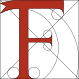
\includegraphics[height=2cm]{F.pdf}
\end{center}


\begin{prose}
J’ai souvenir que, pour se rendre à un mariage, elle voulut se faire les sourcils. Je lui suggérai alors de ne les refaire qu’à la condition de conserver cette encoche si singulière.
\end{prose}

\poemtitle[L’exhortation de Ȝumār par le sourcil fendu]{L’exhortation de \fallbackserif{\textbf{Ȝ}}umār\endnote{On rapporte que l’apôtre Ȝumār a annoncé \enquote{Apprenez à vos enfants l’archerie, la natation, et l’équitation}. Or, chaqu’une des trois premières strophes de ce poème s’attache à l’une de ces disciplines} par le sourcil fendu}
\begin{verse}
Le sourcil fendu à la pointe double\\
Qui s’encoche à l’arcade sourcière\\
Bandée par la mydriase si singulière\\
Me prend pour cible et me trouble,

Me projette sur les eaux d’un océan.\\
Par les deux pans qui sont les sillons,\\
D’une brasse haletante mais pélage\endnote{Hapax dû à la licence poétique. De \autonym{pélagique}, \enquote{de haute mer}.}\\
Me fait échoir épuisé sur le rivage

Où une jument fouette de sa queue\\
Qui, dans le vent, se scinde en deux.\\
La chevauchant, Zulfixār\endnote{Épée à pointe double que Mahomet a trouvé dans le butin de la bataille de Badr.} en main,\\
Elle m’entraine jusqu’au lointain.

Mystère de la disgrâce qui se fit victoire.\\
Surlignant de l’encre pileuse l’iris \xenism{barroco}\endnote{Du portugais \xenism{barroco}, désigne en joaillerie une pierre belle parcequ’irrégulière.}\label{foot.barroco},\\
Kintsungi\endnote{Du japonais 金継ぎ \enquote{jointure d’or}, désigne une technique de céramique brisée dont en suite les morceaux sont rassemblés par une jointure d’or, lui conférant un plus bel aspect que si elle était intacte. À rapprocher de la note \ref{foot.barroco}.} rendit-elle le mammaire ivoire\\
Entrainant les vibrations de mes pectoraux.
\end{verse}


\poemtitle{Un sourire et j’anhéle}
\begin{verse}
Sourire qui projette les aurores radiales\\
Puis retrousse et affine le bourrelet labial\\
De ses commissures qui se renâclent,\\
Saisit mes pectoraux et élargit le thorax.

D’un sentiment haletant,\\
Qui aspire l’air ambiant,\\
L’engouffre dans les poumons,\\
Et l’expire promptement.
\end{verse}

\poemtitle{La faufilade sous le chemisier}
\begin{verse}
Souple est l’orbe voluptueux,\\
Serti du rubis le plus précieux.\\
Porté en avant, orgueilleux et galbé,\\
Il est de la reine la fierté.

Tenu en main, son verni de velours\\
Submerge de la languissante volupté\\
Et s’en va alors fleurir et enfler\\
Car de tendresse flatté à son tour.

Hallebardier est l’outremer chemisier,\\
Celui aux pépites d’or parsemé,\\
Sous lequel une herse sévère entrave,\\
Avec de l’amante le regard grave.

Sur les tours cylindres\endnote{Voir note \ref{foot.tourRonde}.}, les assauts font défection\\
Mais autour de l’imprenable citadelle sphérique,\\
La belle rotondité accroit l’arduité mégalithique,\\
Dont les attraits obstinent cependant l’assaillant.
\end{verse}


%\paragraph{}
\begin{prose}
Ce poème écrit en maghrebi, le dialecte marocain, langue qui \caution{malgré son apparente ressemblance avec l’arabe littéral du fait de quantité de racines, tiendrait davantage du carthaginois}.

Il aborde dans un style proche du genre musical ca\fallbackserif{ȝ}bi \incise{que j’honni pourtant} des thèmes enracinés dans un tropisme marocain et sans doute même passéiste. Mais dont les préoccupations animent à s’y méprendre les contemporains.

La traduction qui en est donnée, qu’après réflexions je voulu davantage littérale quoique s’accommodant de quelques adaptations plus littéraires, trahis forcément les rîmes et la métrique.
J’avais pourtant fermement songé à rendre le texte maghrébi par un équivalent littéraire qui sacrifierais sans hésiter le sens pour ne conserver que l’exaltation qui en est ressentie. Choix auquel j’ai, sans doute à tort, fini par renoncé.
\end{prose}

\poemtitle{Zajal d’un insomniaque épris — \textarabic{زجل العشّاق الصهران}}


\begin{longtable}{R{0.3\textwidth} L{0.65\textwidth}}

\textarabic{أنا بالليل}                  &       Dans mes nuits,   \\
\textarabic{حاضي الگمرا لا تطير.}         &       Je veille à ce que la lune ne croule.   \\
\\
\textarabic{ضال فايق،}                   &       Demeurant éveillé,   \\
\textarabic{و فبالي صوت الضقايق،}        &       L’esprit des percutions de cuivre imbibé,   \\
\\
\textarabic{راني خايف}                   &       Je crains   \\
\textarabic{لَي جي يقجني السّالف}          &       Que la longue natte vienne m’étrangler   \\
\\
\textarabic{و معا الغربي،}               &       Et avec le zéphyr,   \\
\textarabic{يطيّر ما باقى دنعاسي.}        &       Sera ravi ce qui me reste de sommeil.   \\
\\
\textarabic{نفكّر فالغزال}                &       Je songe à la belle   \\
\textarabic{لي گع ميخطى البال.}          &       Qui ne quitte jamais mes pensées.   \\
\\
\textarabic{منفخا عليىا}                 &       Me dédaignant,   \\
\textarabic{و متخصر حتا شوفى فيا.}       &       Elle ne m’accorde pas un seul regard.   \\
\\
\textarabic{ورى الشبيك}                  &       À travers le moucharabieh   \\
\textarabic{ما تورّي لجيهتي غير الشيك}    &       Elle ne me laisse paraitre que la superbe   \\
\\
\textarabic{وخى هكّاك،}                   &       Et malgré tout,   \\
\textarabic{من الشريكة متبوس الحناك.}    &       De la rivale elle n’embrasses pas les joues.   \\
\\
\textarabic{مولات التاج}                  &       La dépositaire de la couronne,   \\
\textarabic{إلى سمعات غيرها تعواج.}      &       Si elle vient à entendre autre qu’elle, se contrarie.   \\
\\
\textarabic{گع النهار،}                  &       Toute la journée,   \\
\textarabic{منها ما نشوف غير الضهر.}     &       Je ne perçois d’elle que le dos.   \\
\\
\textarabic{بكترت ما جميل}               &       Par tan de beauté,   \\
\textarabic{شعرها الكحل غلب الليل}       &       Ses cheveux noirs vainquent la nuit.   \\
\\
\textarabic{طول من النّيل}                &       Plus long que le Nil,   \\
\textarabic{و ضلامو يطفي الپيل}          &       Son obscurité éteint la lampe-torche   \\
\\
\textarabic{ولات فطحا}                    &       Plate est devenue   \\
\textarabic{الگمرا فحضره گلستها المالحا} &       La lune à l’avènement de son assise raffinée   \\
\\
\textarabic{الزيف الريض (الحمر)}         &       Si le voile \xenism{red} (rouge)   \\
\textarabic{الا مشا حتا زلق نفيض}         &       Vient à glisser, je fond.   \\
\\
\textarabic{لعندي،}                      &       Vers moi,   \\
\textarabic{راهى حالفا ربي لا تجي.}       &       Elle jure par Dieu de ne jamais venir.   \\
\\
\textarabic{بلا كوڤيد}                    &       Sans covid,   \\
\textarabic{فراقها خلاني مريض}            &       La séparation me laisse malade. \\
\\
\textarabic{معا ليالي،}                  &       Avec mes nuits,   \\
\textarabic{دّات لي حتى قلبي.}            &       Elle a emporté jusqu’à mon cœur.   \\
\\
\textarabic{تا من العقل}                 &       Et mon encéphale aussi   \\
\textarabic{ولّا كي الآلة فالمعمل.}        &       Est devenu tel l’engin de l’usine.   \\
\\
\textarabic{يضل يخدم}                    &       Il demeure en fonction   \\
\textarabic{ميمشي منو الهمّ.}             &       Et ne se défait de l’anxiété.   \\
\\
\textarabic{شغادي يصنع}                  &       Qu’escompte produire   \\
\textarabic{لي حتا امّ الربيع ميقطع؟}     &       Ce qui ne traverse le fleuve d’Um al~rabiȝ ?   \\
\\
\textarabic{لي بغي يزيد}                 &       Celui qui s’avance   \\
\textarabic{من مهديه لسيدي بوزيد}        &       De Mehdia vers Sidi~Bouzid \\
\\
\textarabic{يبقى يتجّر}                   &       Demeure entrainé   \\
\textarabic{فاليل حتى يودّن الفجر.}       &       Dans la nuit jusqu’à ce que retentisse  l’aurore.   \\
\\
\textarabic{ربي العالي}                  &       Grand Dieu,   \\
\textarabic{بغيت منها غير الشفاري}       &       Je n’espère d’elle que les paupières   \\
\\
\textarabic{و إلى ما لقيتها}             &       Et si je ne la trouve pas,   \\
\textarabic{نضلّ نقلّب على القافية}        &       Je poursuivrais la recherche des rîmes   \\
\end{longtable}

\poemtitle{La voir dans la nuit}
\begin{verse}
L’ardeur qui me pousse à l’admirer malgré la nuit\\
Contraint ma perception à la nyctalopie,\\
Si bien qu’en son absence tout parait odieux\\
Et y est préférable de se crever les yeux.
\end{verse}

\begin{prose}
Dans un café, J’attendais F***. Un signe de sa part. Tandis que le temps passait, des noix de palmiers tombaient à intervalle plus ou moins régulier, comme pour ponctuer le défilement du temps.
\end{prose}

\poemtitle{L’absence}
\begin{verse}
Gorgée après gorgée,\\
Mon verre s’est vidé.\\
Et l’anse ne saurait,\\
À tes bras, suppléer.
%Et l’anse ne saura\\
%tes bras substituer\\
~
\emph{Ô yeux, ô nuit, ô nuit, ô yeux.}
~
Ô, voix de plus en plus moindre\\
Qui tombe comme l’averse\\
Ne peut suffire à éteindre\\
Le brasier qui me traverse.
~
\emph{Ô nuit, ô yeux, ô nuit, ô yeux.}
~
Maudit instant où, de mon verre,\\
N’apparaît que fin liseré\\
Où subsiste peu de café.\\
J’ignore en vérité qu’en faire.\\
Assurément qu’à l’achever\\
Je me résoudrais que par fer.
~
\emph{Ô yeux, ô nuit, ô yeux, ô nuit.}
~
Le palmier qui laisse échoir ses noix,\\
Dont la pourtant sévère  cadence\\
Rappelle ta si pénible absence,\\
À mes cotés pleure mon désarrois.
~
\emph{Ô nuit, ô nuit, ô yeux, ô yeux.}
~
Lorsqu’avec grande flagrance, ton rôle\\
Dissone d’avec tes rares paroles\\
Pour quels choix, dis-moi, puis-je encore opter\\
Tandis que tu ne veux t’en expliquer ?
~
\emph{Ô nuit, ô yeux, ô yeux, ô nuit.}
~
Concède et pardonne\\
Qu’aux yeux me fixant\\
Gorgés d’océans\\
Je m’ abandonne
~
\emph{Ô yeux, ô nuit, ô nuit, ô yeux.}
~
Toi qui ailleurs dirige le mât\\
En fait de tout louvoyant discours,\\
Si tu dubites de mon amour,\\
Regarde ma vulve et tu saura.
\end{verse}

\poemtitle{Du naufrage}
\begin{verse}
J’ai perdu ma proue
Et mon navire a coulé,
Dans l’eau, tout entier.
\end{verse}

\begin{prose}
Me trouvant non loin du musée de Bank-al-Maghrib, je me dis qu’il valait encore mieux y noyer ma peine. Grand bien me pris car alors \incise{joi} bien loin de m’en douter, j’y trouvais des éléments prélevés sur le site archéologique d’Aghmat, des parties de la maison d’Al\,Mutamid Ibn~Abbad qui commandita à Lissān~al\,Ḋḋīne ibn~al\,Xatīb des poèmes à graver sur ses murs. Mais plus bouleversant encore, un manuscrit que je crus comprendre autographe de Lissān~al\,Ḋḋīne ! Fort heureusement, le masque que je portais du fait de l’épidémie m’épargna le ridicule d’exposer aux gens les larmes qui coulèrent le long de mes joues. Je me suis même retenu de m’assoir par terre tant me jambes s’étaient vidées de leur tonus.

Je dois toute fois être honnête, je n’ai pas pris la peine de vérifier que les manuscrits étaient bien autographes comme j’ai cru le comprendre ; ou plus exactement j’ai soigneusement évité de m’en assurer, préférant me complaire dans l’idée qu’ils l’étaient.
\end{prose}

%\paragraph{}
\poemtitle[Le Zurbiy]{Le \xenism{Zurbiy}\endnote{Le dernier sultan de Grenade, Mohammed XII de Grenade, dit al\,Zurbiy \xenism{l’infortuné} fut le dernier souverain musulman d’al\,Andalus.}}
\begin{verse}
Comme un prince de son royaume banni,\\
Qui ne reverra plus  son Andalousie,\\
De notre amour, l’échec et mat\\
M’est aussi odieux qu’Aghmat.\endnote{Al\,Mutamid Ibn~Abbad  qui a été roi de Séville, fût destitué par les Almoravides pour être exilé à Aghmat où il mourus.}
~
Que vienne me voir le double-visir\endnote{Allusion à Lissān~al\,Ḋḋīne ibn~al\,Xatīb, savant qui fut par deux fois ministre aux cours nasride et mérinide, ce qui lui valut le surnom de \enquote{celui aux deux visirat} \textarabic{ذي الوزارتين}. Lors de son exil à Aghmat, Al\,Mutamid Ibn~Abbad fit appel à ses services de poète pour rédiger des vers qui furent calligraphiés sur les murs de sa maison.}\\
Et qu’avec ses royaux vers enchanteurs,\\
Ceux qui sont gravés loin sur les hauteurs,\\
Soit marquée l’extinction du désir.
\end{verse}

\section*{Didactique}
\addcontentsline{toc}{section}{Didactique}

\begin{prose}
Il y’avait, je ne me souviens plus quand exactement, un enfant à qui je devais, pour lui donner un cours de langue, lui illustrer que notre langue n’est pas à la vérité des plus aisée. Je lui donnais l’exemple des mots du cheval et la grande variété des racines pour les former.
\end{prose}


\poemtitle{Les mots du cheval}
\begin{verse}
Prenons un animal,\\
au hasard, le \autonym{cheval}.
~
Sa femelle, la \autonym{jument}\\
Est une douce maman.
~
Elle fait des câlins\\
À son petit \autonym{poulain}.
~
Si jamais on le fait \autonym{hongre},\\
il deviendra castré, bigre !
~
S’il en est autrement,\\
Il sera \autonym{étalon}.
~
Luttant avec fierté,\\
Il sera le \autonym{destrier}
~
Ou distant de l’effroi\\
En charmant \autonym{palefroi}.
~
Scellé par un \autonym{écuyer},\\
Il mène le \autonym{cavalier}.
~
Ou au jeu de la paix,\\
Par le beau \autonym{jokey}
~
Dans une course \autonym{hippique}\\
Qui sera aussi épique
~
Que nous croyons souvent\\
Être \autonym{équitation}.
~
Ferres-toi auparavant\\
Par le \autonym{maréchal-ferrant}
\end{verse}



\section*{Courtes épopées d’arc et de dague}
\addcontentsline{toc}{section}{Courtes épopées d’arc et de dague}
\poemtitle{Exorde à l’archer}
\begin{verse}
Tapisse toi derrière le merlon et encoche\\
La flèche perçant le catafractaire en approche.\\
Tiens-toi devant le créneau et libère\\
La flèche traçant la cuirasse fière.

Dégaine l’épée à la lame damascène,\\
Suspends-en promptement de l’assaillant l’allène.\\
Et le sang qui ruissellera sur le moiré,\\
Séché, sera donc legs à la postérité.

Les faisceaux indéfectibles, par la guivre,\\
Seront noués de sa dépouille languide.
Exorde aux justes de s’y rallier
Et rappel de l’engeance terrassée.
\end{verse}

\poemtitle{Les dagues des meurtrières}
\begin{verse}
Les cheveux bouclés qui flottent au vent\\
Sont la bannière de celles aux charmes ondulants.\\
Coiffées d’autant de dagues meurtrières,\\
Donnant l’ennemi aux sinuosités de la guerre.
\end{verse}

\poemtitle{Le sang ennemi}
\begin{verse}
Que toujours dans nos coupes, vermeils se déversent\\
Les torrent affluents des  régiments occis.\\
Que toujours dans nos coupes, le sang ennemi\\
Pleuve jusqu’au buvant et remplisse en averses.
\end{verse}

\section*{Vers d’autres horizons}
\addcontentsline{toc}{section}{Vers d’autres horizons}

\poemtitle{Laurier éclatant}
\begin{verse}
Le laurier qui explose en mille émotions,
Lance ses fleures en toutes directions,
Sous lesquelles les rayons du soleil s’infiltrent,
Et de l’astre lumineux apportent l’épitre.
\end{verse}

\begin{prose}
  Je tâchais dans ce recueil de poèmes tout au long de sa composition de demeurer simple. Après tout, Sun Tzu ne dit-il pas si bien :

  \begin{quotation}
    Il arrive qu’étant parvenu à se hisser jusqu’au bon, l’on puisse aller encore au delà. Mais ce qui est au dessus du bon n’est point le bon lui même.
  \end{quotation}

  Je ne sais si j’y suis parvenu mais au moins, je m’y serais efforcé.
\end{prose}

\begin{prose}
Que dire encore, sinon que je me souviens que lorsque F*** m’emmena sur les remparts de la cité portugaise à Eljadida, elle m’entraina jusqu’à un mirador où notre intimité ne fût rompue que par un rayon de lumière.
\end{prose}

\poemtitle{Ruban de lumière}
\begin{verse}
Un éphémère ruban fait de lumière
Se faufila à travers la meurtrière
Et alla se nouer autour des cheveux
Aux complexe réseau de mèches en feux.
\end{verse}

\poemtitle{Matins éternels}
\begin{verse}
Si ce matin-là était beau à m’en rendre ivre,
De tels, il y en eu tant avant que je naisse,
Il y aura après que j’ai cessé de vivre.
Des beauté du monde je n’aurais pas vu once.
\end{verse}

\poemtitle{La paix}
\begin{verse}
Écoutez ! La harpe d’Hathor\endnote{Déesse égyptienne de la musique, de l’amour, et de la joie.} est libérée.\\
Seul le cliquetis de la lance métallique\\
Est instrument lorsqu’il est à terre tombé.\\
Tandis que s’étreignent les corps diplomatique.

Archer, noue ta corde à cette cheville\\
Avec l’oud rejoins l’orchestre sacré\\
Qui commémore la guerre achevée\\
Quand d’allégresse la fille trésaille.

Défaisant les sangles corsetant le pied\\
De ses sandales elle s’est délestée\\
Et dans la marrée elle mouille la jambe\\
D’un mouvement frêle, souple et ingambe

Monte plus haut réverbe de l’aulos\\
Dont la Divinité est le présent\\
Nous éloignant à jamais de l’atroce\\
Par ses parfums exquis et apaisants.

Que les paupières se ferment entrainées par les cils\\
Alourdis des gouttelettes qui abreuvent le Nil\\
De ses généreux torrents d’eau fraîche et intarissable\\
Semblant chaudes lorsqu’elles aspergent nos corps aimables
\end{verse}
